\documentclass[12pt]{article}
\usepackage[margin=1.5cm]{geometry}
\usepackage{parskip}
\usepackage{amsmath}
\usepackage{amssymb}
\usepackage{amsfonts}
\usepackage{enumitem}
\usepackage{graphicx}
\usepackage{stmaryrd}
\graphicspath{ {./images/} }


\begin{document}

The Nussinov algorithm is an algorithm to compute RNA secondary structure, i.e. where the RNA pairs with itself. This is useful because it can indicate cell function.

The Nussinov algorithm is a dynamic programming algorithm. The idea behind it is that the optimal structure for an RNA sequence can be found by combining optimal substructures.

The optimal substructure $[i,j]$ must be formed from one of the following mechanisms:


\begin{itemize}
    
  \item
Having $i,j$ paired
\item

Having $i$ unpaired
\item

Having $j$ unpaired
\item

Combining two optimal substructures through bifurcation.
\end{itemize}

The algorithm takes as input a single RNA sequence, and outputs the optimal secondary structure.

The dynamic programming function looks like the following:

\[
  \gamma(i,j) = \max \begin{cases}\gamma(i+1, j-1) + \delta(i,j)\\\gamma(i+1, j) \\\gamma(i, j-1)\\\max_{i < k < j} (\gamma(i,k) + \gamma(k+1, j)\end{cases}
.\]

Where $\delta(i,j) = 1$ if $i,j$ are complementary, and 0 otherwise.

We initialise with $\gamma(i, i-1) = 0$ and $\gamma(i,i) = 0$ for all $i$ representing sequences of length $0$ and $1$.


As an example, consider finding the optimal structure for sequence CAGACUG

We get the following matrix:

\begin{tabular}{c|c|c|c|c|c|c|c|c}
  &$\omega$&C&A&G&A&C&U&G\\
  \hline
  C&0&0&0&1&1&1&2&3\\
  \hline
  A&&0&0&0&0&1&2&2\\
  \hline
  G&&&0&0&0&1&1&1\\
  \hline
  A&&&&0&0&0&1&1\\
  \hline
  C&&&&&0&0&0&1\\
  \hline
  U&&&&&&0&0&0\\
  \hline
  G&&&&&&&0&0
\end{tabular}

This yields the following structure:

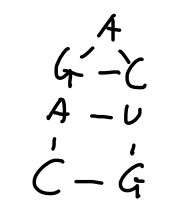
\includegraphics[scale=0.5]{rnastructure}

This algorithm has time complexity $O(n^3)$ (with $n$ being the length of the input sequence). This is because we must fill half of an $n \times n$ matrix, where filling each cell takes time $O(n)$ (due to the bifurcation mechanism), giving us $O(n^3)$ time complexity.

It has space complexity $O(n^2)$ to store the matrix.

The algorithm has a few flaws. For example, it only considers 2D structure, whereas RNA will actually exist in 3 dimensions. Furthermore, it does not allow for RNA pseudoknots, i.e. when one base pairs with two other bases.





    
\end{document}
